\chapter{肌肉收缩与运动功能}\label{ch:b2:muscle-movement}

一名短跑运动员起跑时，作用于跑道的力
可达其体重的三倍，在五分之一秒内由此前还松弛的肌肉产生。
细胞本身并未缩短：
细丝在细胞内相互滑过，由数以百万计的分子“手”牵引，
每只“手”迈出约十纳米的一步后松开，
每秒循环十次，每次消耗一个 ATP。本章
承接\cref{ch:b2:cell-differentiation}中的\omterm{def:b2:cell-differentiation:myogenesis}{肌纤维}，讨论它如何工作：
细丝的滑动，以及驱动滑动的分子马达，
钙开关如何开启与关闭马达，神经发出的指令，
力与速度的力学，
以及神经系统如何调控这一切，
从\omterm{def:b2:muscle-movement:motorunit}{单收缩}直至冲刺。

\section{滑动的细丝}

\begin{proposition}[肌丝滑动机制]\label{prop:b2:muscle-movement:sliding}
\index{肌丝滑动}\index{肌节!收缩}
\omterm{def:b2:cell-differentiation:myogenesis}{肌纤维}缩短时，其\omterm{def:b2:cell-differentiation:fibre}{肌节}随之缩短
（见\cref{ch:b2:cell-differentiation}），但粗肌丝（\omterm{prop:b2:muscle-movement:crossbridge}{肌球蛋白}）
与细肌丝（肌动蛋白）的长度都不改变：细丝
沿粗丝向内滑动，I 带与 H 区变窄，Z 盘相互靠近。
两组丝的重叠区即产生力之处，\omterm{def:b2:cell-differentiation:fibre}{肌节}产生的力
与重叠成正比：
从拉伸长度 \qty{3.6}{\micro m} 起，此时无重叠、无力，
随细丝重叠增多，力线性上升，
在 \qty{2.2}{\micro m} 附近达到平台，此时每个\omterm{prop:b2:muscle-movement:crossbridge}{肌球蛋白}头部都面向肌动蛋白，
低于 \qty{2.0}{\micro m} 后又下降，
细丝相互碰撞，粗丝撞上 Z 盘。体内肌肉的
静息长度恰位于平台上，
这正是力如何产生的
第一条线索。
\end{proposition}
\begin{proof}[证据]
A.~F.~赫胥黎与尼德格克，以及 H.~E.~赫胥黎与汉森（1954 年）
用干涉与相差显微镜观察单根\omterm{def:b2:cell-differentiation:myogenesis}{肌纤维}及分离\omterm{def:b2:cell-differentiation:fibre}{肌原纤维}缩短时的各带：
A 带长度不变，I 带缩短，故细丝滑动。戈登、赫胥黎与朱利安
（1966 年）将单根\omterm{def:b2:cell-differentiation:myogenesis}{肌纤维}固定在设定长度，
并以反馈装置使一段\omterm{def:b2:cell-differentiation:fibre}{肌节}长度保持恒定，
发现力与粗、细丝重叠程度成正比，
重叠程度经电子显微镜测得——即长度—张力曲线
具有平台与两段线性支，
与丝的几何结构所预示的
完全一致。
\end{proof}

\begin{omfigure}
\begin{minipage}[b]{0.5\linewidth}\centering
\begin{tikzpicture}[every node/.style={font=\scriptsize}]
  \foreach \y/\lab/\ov in {2.4/{舒张，\qty{2.6}{\micro m}}/0.9, 1.2/{收缩，\qty{2.0}{\micro m}}/0.3} {
    \begin{scope}[yshift=\y cm]
      \draw[very thick, omThm] (0,-0.35) -- (0,0.35); \draw[very thick, omThm] (4.4-2*\ov+1.0,-0.35) -- (4.4-2*\ov+1.0,0.35);
      \pgfmathsetmacro{\len}{4.4-2*\ov+1.0}
      \foreach \dy in {-0.25,0.05,0.25} { \draw[thick, omDef] (0,\dy) -- (1.5,\dy); \draw[thick, omDef] (\len,\dy) -- (\len-1.5,\dy); }
      \draw[line width=3pt, omExo!80!black] (\len/2-1.1,-0.1) -- (\len/2+1.1,-0.1);
      \node[right] at (\len+0.15,0) {\lab};
    \end{scope}
  }
  \node[align=center] at (2.7,0.1) {肌丝长度保持不变；\\重叠区随 Z 盘靠近而增大};
\end{tikzpicture}
\end{minipage}\hfill
\begin{minipage}[b]{0.48\linewidth}\centering
\begin{tikzpicture}
\begin{axis}[
  width=\linewidth, height=4.8cm,
  axis x line=bottom, axis y line=left,
  xmin=1.2, xmax=3.8, ymin=0, ymax=1.15,
  xlabel={肌节长度 (\unit{\micro m})}, ylabel={力（相对值）},
  xlabel style={font=\scriptsize, at={(axis description cs:0.5,-0.17)}, anchor=north},
  ylabel style={font=\scriptsize},
  tick label style={font=\scriptsize}, xtick={1.3,2.0,2.2,3.6}, ytick={0,0.5,1},
  clip=false,
]
\addplot[very thick, omDef] coordinates {(1.3,0) (1.65,0.5) (2.0,1) (2.2,1) (3.6,0)};
\node[font=\scriptsize, anchor=south] at (axis cs:2.1,1.02) {平台期};
\node[font=\scriptsize, anchor=west, align=left] at (axis cs:2.95,0.75) {重叠 \\减少};
\end{axis}
\end{tikzpicture}
\end{minipage}

{\small 左：舒张与收缩状态的\omterm{def:b2:cell-differentiation:fibre}{肌节}——细肌丝（蓝色）
沿粗肌丝（灰色）滑动而长度不变。右：长度—张力曲线，
力与重叠程度成正比，
在静息肌肉所处的平台期最大。}
\end{omfigure}

\begin{omfigure}
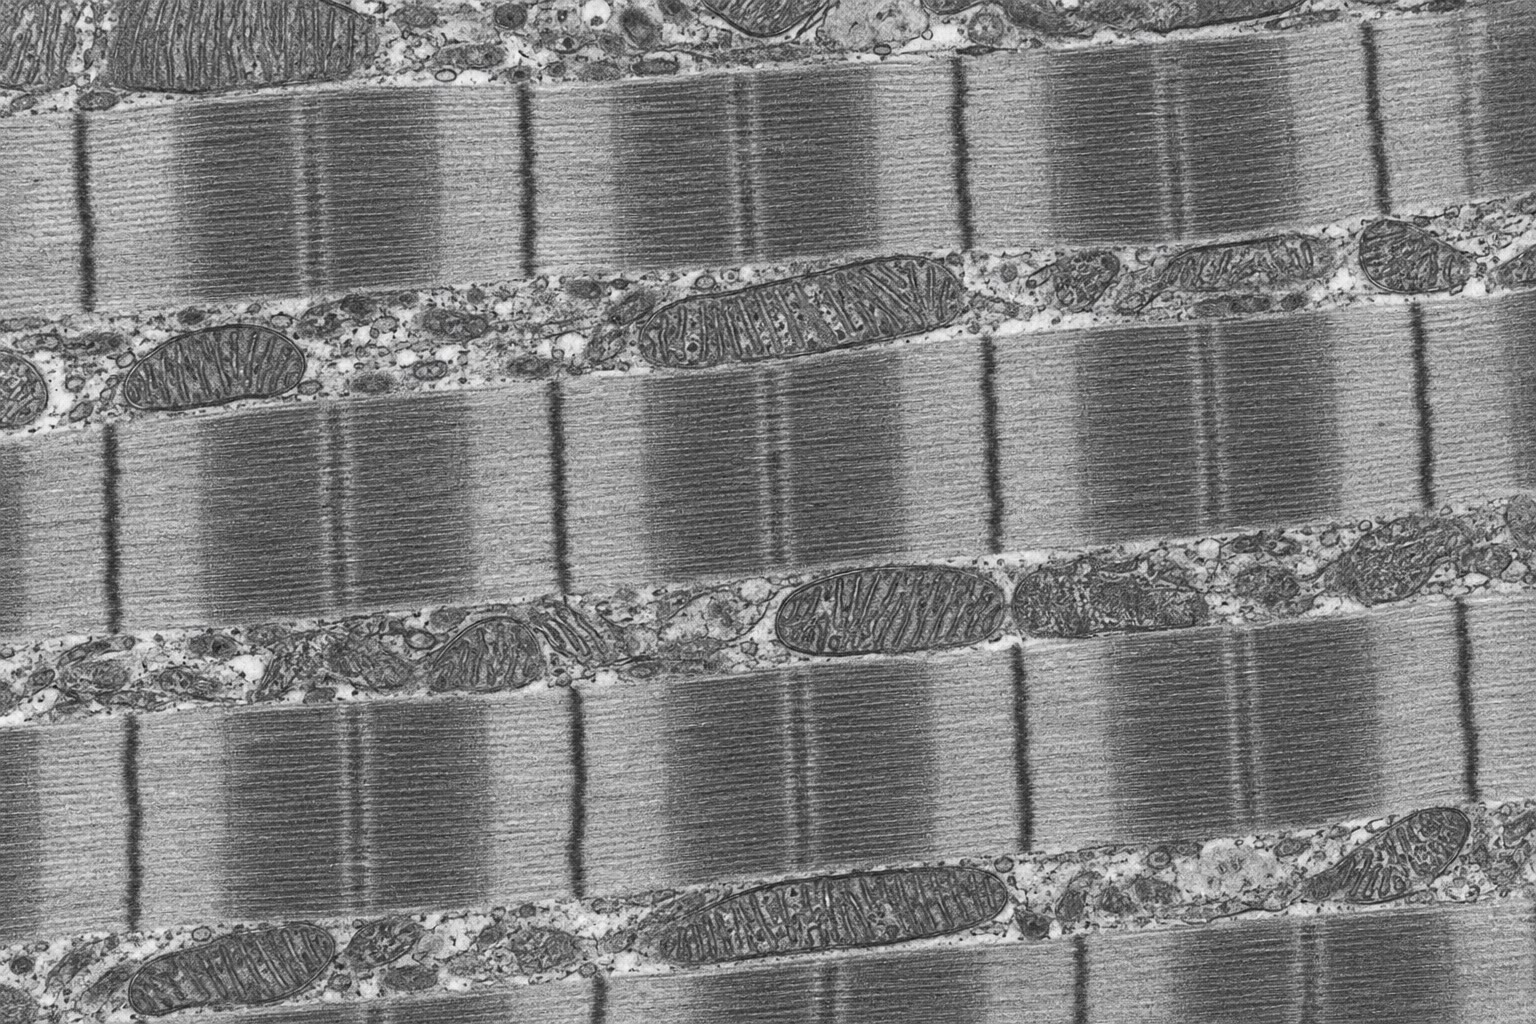
\includegraphics[width=0.6\linewidth]{images/book4/ai/b4-21-sarcomere-tem.jpg}

{\small 电镜下的\omterm{def:b2:cell-differentiation:fibre}{肌原纤维}：粗肌丝所在的 A 带、
细肌丝所在、被 Z 线平分的 I 带，
以及为滑动提供能量的\omterm{def:b2:cell-differentiation:fibre}{肌原纤维}间线粒体。}
\end{omfigure}

\section{分子马达}

\begin{proposition}[横桥循环]\label{prop:b2:muscle-movement:crossbridge}
\index{横桥循环}\index{肌球蛋白}\index{ATP!在收缩中}
每根粗肌丝上约有三百个\emph{\omterm{prop:b2:muscle-movement:crossbridge}{肌球蛋白}头部}，
每个头部都是一台沿肌动蛋白行走的分子马达，
循环分为四步。（1）结合 ATP 时，头部与肌动蛋白脱离；
头部将 ATP 水解为 ADP 与磷酸，并扳成
紧张的高能构象。（2）扳起的头部结合一个肌动蛋白亚基，
形成\emph{横桥}。（3）磷酸释放，头部弹回松弛构象，
将细肌丝拉向\omterm{def:b2:cell-differentiation:fibre}{肌节}中央约 \qty{10}{nm}，
即\emph{动力冲程}；ADP 脱落。（4）新的 ATP 结合，
头部与肌动蛋白脱离；无 ATP 时头部无法脱开，
这就是死后僵直的原因。
一次循环约需二十分之一秒，头部大部分时间处于脱离状态，
因此任一时刻只有一部分头部在拉动，
高速滑动的细丝始终不会失去连接。
力是结合头部拉力之和；缩短量是各步之和，
每个\omterm{def:b2:cell-differentiation:fibre}{肌节}每循环至多缩短半微米；
能量方面，每个头部每步消耗一个 ATP，
约 \qty{50}{kJ/mol}——即每步 \qty{8e-20}{J}，
其中头部至多将一半转化为功。
\end{proposition}

\begin{omfigure}
\begin{tikzpicture}[every node/.style={font=\scriptsize}, >=stealth]
  \foreach \x/\lab/\ang/\att in {0/{1. 结合 ATP：\\头部脱离；ATP\\水解，头部翘起}/60/0, 3.6/{2. 翘起的头部 \\结合肌动蛋白：\\形成横桥}/60/1, 7.2/{3. 释放磷酸：\\动力冲程，\\细丝被拉动 \qty{10}{nm}}/20/1, 10.8/{4. ADP 离开，新的 \\ATP 结合：头部 \\松开}/20/0} {
    \begin{scope}[xshift=\x cm]
      \draw[thick, omDef] (0,2.2) -- (2.8,2.2); \foreach \i in {0.2,0.6,...,2.6} \fill[omDef!50] (\i,2.2) circle (0.14);
      \draw[line width=3pt, omExo!80!black] (0,0.4) -- (2.8,0.4);
      \draw[very thick, omThm] (1.4,0.4) -- (1.4,1.0);
      \ifnum\att=1 \draw[very thick, omThm] (1.4,1.0) -- ++(\ang:1.15); \fill[omThm] (1.4,1.0) ++(\ang:1.15) circle (0.16); \else \draw[very thick, omThm] (1.4,1.0) -- ++(\ang:1.0); \fill[omThm] (1.4,1.0) ++(\ang:1.0) circle (0.16); \fi
      \node[below, align=center] at (1.4,0.15) {\lab};
    \end{scope}
  }
  \draw[->, thick, omDef] (7.9,2.55) -- (8.9,2.55); \node[omDef, above] at (8.4,2.6) {细丝移动};
\end{tikzpicture}

{\small \omterm{prop:b2:muscle-movement:crossbridge}{横桥循环}。蓄力构象的\omterm{prop:b2:muscle-movement:crossbridge}{肌球蛋白}头部（红色）结合
肌动蛋白（蓝色），释放磷酸基团，通过动力冲程拉动细丝，
随后结合新的 ATP 并松开。}
\end{omfigure}

\begin{theorem}[肌肉的力、速度与功率]\label{thm:b2:muscle-movement:hill}
\index{力–速度曲线}\index{肌肉功率}
肌肉的力随缩短速度加快而下降，原因在于细丝滑动越快，
任一时刻结合的头部越少，
而在松开之前被拖过冲程的头部越多。
希尔关系式描述了这一关系：
\[
(F + a)(v + b) = (F_0 + a)\,b,
\]
其中 $F_0$ 为等长收缩力（$v = 0$ 时），$v_{\max} =
F_0 b/a$ 为空载速度，$a$、$b$ 为常数（$a \approx
F_0/4$）。功率 $Fv$ 在两端为零，最大值约出现在
$v_{\max}$ 的三分之一、$F_0$ 的三分之一处——这正是骑车人
要换挡、短跑运动员步幅有偏好频率的原因。人体肌肉
每平方厘米横截面约能产生 \qty{30}{N} 的力，
每秒最多可缩短十个自身长度，并
在最佳状态下每千克可输出约 \qty{100}{W} 的功率。
\end{theorem}
\begin{proof}
希尔曲线是经验性的（1938 年），在离体蛙肌上测得
缩短速度与所提起负荷之间的关系；双曲线形式的成立
是因为结合头部的比例随滑动速度下降，
且每个结合头部的力随其经历冲程而减小。
功率：由 $F = (F_0 + a)b/(v + b) - a$，$Fv$ 在
$v = 0$ 与 $v_{\max}$ 处为零；求导得最大值位于
$v = b(\sqrt{(F_0 + a)/a} - 1)$，当 $a = F_0/4$ 时，$v =
1.24\,b = 0.31\,v_{\max}$，此时 $F = 0.31\,F_0$。
\end{proof}

\begin{omfigure}
\begin{tikzpicture}
\begin{axis}[
  width=0.7\linewidth, height=5.4cm,
  axis x line=bottom, axis y line=left,
  xmin=0, xmax=1.05, ymin=0, ymax=1.1,
  xlabel={缩短速度 $v/v_{\max}$}, ylabel={力 $F/F_0$，功率（相对值）},
  xlabel style={font=\small, at={(axis description cs:0.5,-0.13)}, anchor=north},
  ylabel style={font=\small},
  tick label style={font=\small}, xtick={0,0.31,1}, xticklabels={0,0.31,1}, ytick={0,0.31,1}, yticklabels={0,0.31,1},
  legend style={font=\scriptsize, at={(0.97,0.95)}, anchor=north east, draw=none},
  clip=false,
]
\addplot[very thick, omDef, domain=0:1, samples=100] {(1.25*0.25)/(x+0.25) - 0.25};
\addlegendentry{力}
\addplot[very thick, omThm, domain=0:1, samples=100] {10.4*x*((1.25*0.25)/(x+0.25) - 0.25)};
\addlegendentry{功率（缩放）}
\draw[dashed, gray] (axis cs:0.31,0) -- (axis cs:0.31,1.0);
\end{axis}
\end{tikzpicture}

{\small 希尔\omterm{thm:b2:muscle-movement:hill}{力–速度曲线}（$a = F_0/4$）及其隐含的功率：
力随肌肉缩短加快而下降，功率峰值出现
在最大速度的约三分之一处，
以及等长收缩力的约三分之一处达到峰值。}
\end{omfigure}

\section{开关：钙}

\begin{proposition}[兴奋–收缩偶联]\label{prop:b2:muscle-movement:coupling}
\index{兴奋–收缩偶联}\index{肌钙蛋白}\index{原肌球蛋白}\index{肌质网}
静息时，\omterm{prop:b2:muscle-movement:crossbridge}{肌球蛋白}头部无法接近肌动蛋白：细丝上的结合位点
被\emph{\omterm{prop:b2:muscle-movement:coupling}{原肌球蛋白}}覆盖，它是一条横卧
在肌动蛋白螺旋凹槽中的杆状分子，并由\emph{\omterm{prop:b2:muscle-movement:coupling}{肌钙蛋白}}固定在那里。
开关是钙。\omterm{def:b2:cell-differentiation:myogenesis}{肌纤维}膜上的\omterm{prop:b2:neurons-synapses:ap}{动作电位}
沿横管向内传导，并在横管与\omterm{def:b2:cell-differentiation:fibre}{肌质网}相接的连接处，
打开\omterm{def:b2:cell-differentiation:fibre}{肌质网}的钙释放通道；
钙涌入\omterm{def:b2:cell-differentiation:fibre}{肌原纤维}，
在一毫秒内从 \qty{0.1}{} 升至 \qty{10}{\micro mol/L}，
与\omterm{prop:b2:muscle-movement:coupling}{肌钙蛋白}结合，\omterm{prop:b2:muscle-movement:coupling}{肌钙蛋白}使\omterm{prop:b2:muscle-movement:coupling}{原肌球蛋白}移离结合位点：
头部得以附着，只要钙留存，纤维就持续收缩。
\omterm{def:b2:cell-differentiation:fibre}{肌质网}中的泵消耗 ATP，
在数十毫秒内将钙泵回；\omterm{prop:b2:muscle-movement:coupling}{原肌球蛋白}重新覆盖
位点，纤维松弛。松弛与收缩同样是主动过程，
缺乏 ATP 的肌肉既无法松开头部，
也无法将钙泵回——即死后僵直。
\omterm{def:b2:heart:anatomy}{心脏}采用同样的开关，
但钙经由膜上自有的通道从外部进入以触发释放，
这正是\omterm{def:b2:heart:anatomy}{心脏}而非骨骼肌
对\omterm{def:b2:blood-circulation:blood}{血液}中的钙敏感的原因。
\end{proposition}

\begin{omfigure}
\begin{tikzpicture}[every node/.style={font=\scriptsize}, >=stealth]
  \node[draw, rounded corners, fill=omDef!15, align=center] (nerve) at (0,0) {运动神经 \\冲动};
  \node[draw, rounded corners, fill=omDef!15, align=center] (nmj) at (3.0,0) {神经肌肉 \\接头：乙酰胆碱};
  \node[draw, rounded corners, fill=omDef!15, align=center] (ap) at (6.2,0) {肌肉动作 \\电位，沿 \\横管下行};
  \node[draw, rounded corners, fill=omThm!15, align=center] (ca) at (9.4,0) {Ca$^{2+}$ 自 \\肌质网释放};
  \node[draw, rounded corners, fill=omProp!20, align=center] (tn) at (12.6,0) {肌钙蛋白结合 Ca$^{2+}$，\\原肌球蛋白移动，\\头部附着};
  \node[draw, rounded corners, fill=omExo!25, align=center] (off) at (9.4,-2.2) {泵回 Ca$^{2+}$（耗 ATP）；\\原肌球蛋白重新覆盖肌动蛋白：\\松弛};
  \draw[->, thick] (nerve) -- (nmj); \draw[->, thick] (nmj) -- (ap); \draw[->, thick] (ap) -- (ca); \draw[->, thick] (ca) -- (tn);
  \draw[->, thick] (ca) -- (off);
  \node[below, gray] at (1.5,-0.7) {\qty{0.6}{ms}}; \node[below, gray] at (4.6,-0.7) {\qty{1}{ms}}; \node[below, gray] at (7.8,-0.7) {\qty{1}{ms}};
\end{tikzpicture}

{\small 从神经冲动到力：接头、
\omterm{def:b2:cell-differentiation:myogenesis}{肌纤维}自身的\omterm{prop:b2:neurons-synapses:ap}{动作电位}、钙的释放，
以及肌动蛋白位点的暴露——然后是终止这一切的泵。}
\end{omfigure}

\section{指令与分级}

\begin{definition}[运动单位]\label{def:b2:muscle-movement:motorunit}
\index{运动单位}\index{单收缩}\index{强直收缩}\index{募集}
脊髓中的一个\emph{运动\omterm{def:b2:neurons-synapses:neuron}{神经元}}，其\omterm{def:b2:neurons-synapses:neuron}{轴突}伸向一块肌肉，
并分支支配从几条到上千条\omterm{def:b2:cell-differentiation:myogenesis}{肌纤维}，这些\omterm{def:b2:cell-differentiation:myogenesis}{肌纤维}散布于整块肌肉中；
该\omterm{def:b2:neurons-synapses:neuron}{神经元}与其支配的\omterm{def:b2:cell-differentiation:myogenesis}{肌纤维}合称一个\emph{运动单位}，
是神经系统能够发出指令的最小力量单位。
\omterm{def:b2:neurons-synapses:neuron}{神经元}的每一次冲动，都使该单位的每条\omterm{def:b2:cell-differentiation:myogenesis}{肌纤维}发放一次，
并产生一次\emph{单收缩}：力量先行上升，
约在\qty{30}{ms}内达到峰值，随后在\qty{100}{ms}内衰减，原因在于
钙脉冲很短。接连的冲动使单收缩叠加：
前一次的钙尚未被泵走，下一次便已到来；
每秒约 30 至 50 次冲动时，力量融合为平滑的\emph{强直收缩}，
约为单收缩的三到五倍。
神经系统以两种方式对肌肉的力量分级：一是按每个单位放电的
\emph{速率}，二是按所募集单位的\emph{数目}——
先募集小型、慢速、抗疲劳的单位，
（\emph{大小原则}）：大型快速单位最后募集，仅用于最大用力。
因此，日常活动中的肌肉从来不会全部
激活：其中一部分单位轮流放电，其余单位则休息。
\end{definition}

\begin{omfigure}
\begin{tikzpicture}
\begin{axis}[
  width=0.82\linewidth, height=5.4cm,
  axis x line=bottom, axis y line=left,
  xmin=0, xmax=1.0, ymin=0, ymax=4.2,
  xlabel={时间（s）}, ylabel={力（单收缩 $=$ 1）},
  xlabel style={font=\small, at={(axis description cs:0.5,-0.13)}, anchor=north},
  ylabel style={font=\small},
  tick label style={font=\small}, xtick={0,0.2,0.4,0.6,0.8,1}, ytick={0,1,2,3,4},
  clip=false,
]
% single twitch
\addplot[very thick, omDef, domain=0:0.2, samples=60] {(x<0.02)*0 + (x>=0.02)*4.5*(x-0.02)*exp(-(x-0.02)/0.03)*4.1};
% summation at 10 Hz
\addplot[very thick, omProp, domain=0.25:0.62, samples=200] {(x>=0.25)*4.5*4.1*(x-0.25)*exp(-(x-0.25)/0.03) + (x>=0.33)*4.5*4.1*(x-0.33)*exp(-(x-0.33)/0.03) + (x>=0.41)*4.5*4.1*(x-0.41)*exp(-(x-0.41)/0.03) + (x>=0.49)*4.5*4.1*(x-0.49)*exp(-(x-0.49)/0.03)};
% tetanus at 50 Hz
\addplot[very thick, omThm, domain=0.66:0.98, samples=100] {3.8*(1-exp(-(x-0.66)/0.06))};
\node[font=\scriptsize, anchor=west] at (axis cs:0.09,0.7) {单次冲动：单收缩};
\node[font=\scriptsize, anchor=south] at (axis cs:0.44,2.2) {\qty{12}{Hz}：叠加};
\node[font=\scriptsize, anchor=south] at (axis cs:0.82,3.85) {\qty{50}{Hz}：融合强直收缩};
\end{axis}
\end{tikzpicture}

{\small 按速率对力分级。单个冲动产生\omterm{def:b2:muscle-movement:motorunit}{单收缩}；
每秒十余次的冲动叠加为起伏的力；每秒五十次时
力融合为\omterm{def:b2:muscle-movement:motorunit}{强直收缩}，约为\omterm{def:b2:muscle-movement:motorunit}{单收缩}的数倍。}
\end{omfigure}

\begin{proposition}[反射与脊髓]\label{prop:b2:muscle-movement:reflex}
\index{反射弧}\index{肌梭}\index{牵张反射}\index{交互抑制}
运动\omterm{def:b2:neurons-synapses:neuron}{神经元}是\emph{最终共同通路}：每一条指令，
无论来自皮层还是来自反射，都终止于它。最简单的回路是
\cref{ch:b2:neurons-synapses}中的\emph{\omterm{prop:b2:muscle-movement:reflex}{牵张反射}}：
感觉末梢环绕在肌肉内部的特殊纤维上，这些纤维即
\emph{\omterm{prop:b2:muscle-movement:reflex}{肌梭}}，在肌肉被拉伸时发放冲动，
经一个\omterm{def:b2:neurons-synapses:synapse}{突触}兴奋同一肌肉的运动\omterm{def:b2:neurons-synapses:neuron}{神经元}，并
经一个中间\omterm{def:b2:neurons-synapses:neuron}{神经元}抑制拮抗肌的运动\omterm{def:b2:neurons-synapses:neuron}{神经元}
（\emph{\omterm{prop:b2:muscle-movement:reflex}{交互抑制}}），使肌肉抵抗拉伸——
这是姿势维持的基础，因为每一次摇晃都是某块肌肉被拉伸。
另有一种感受器——腱器官——在肌肉力量较大时发放冲动，
并抑制该肌自身的运动\omterm{def:b2:neurons-synapses:neuron}{神经元}，是一道安全阀。
对疼痛刺激的撤回是一种多\omterm{def:b2:neurons-synapses:synapse}{突触}反射，
使该肢屈曲，同时另一侧的肢体伸展，
以免你跌倒。大脑指挥的并非肌肉，
而是动作：皮层发出计划，小脑依据\omterm{prop:b2:muscle-movement:reflex}{肌梭}的反馈加以校正，
基底神经节释放该计划，
而脊髓的回路（能够自行产生迈步节律）负责执行，
这正是
本科三年级分册的主题。
\end{proposition}

\begin{omfigure}
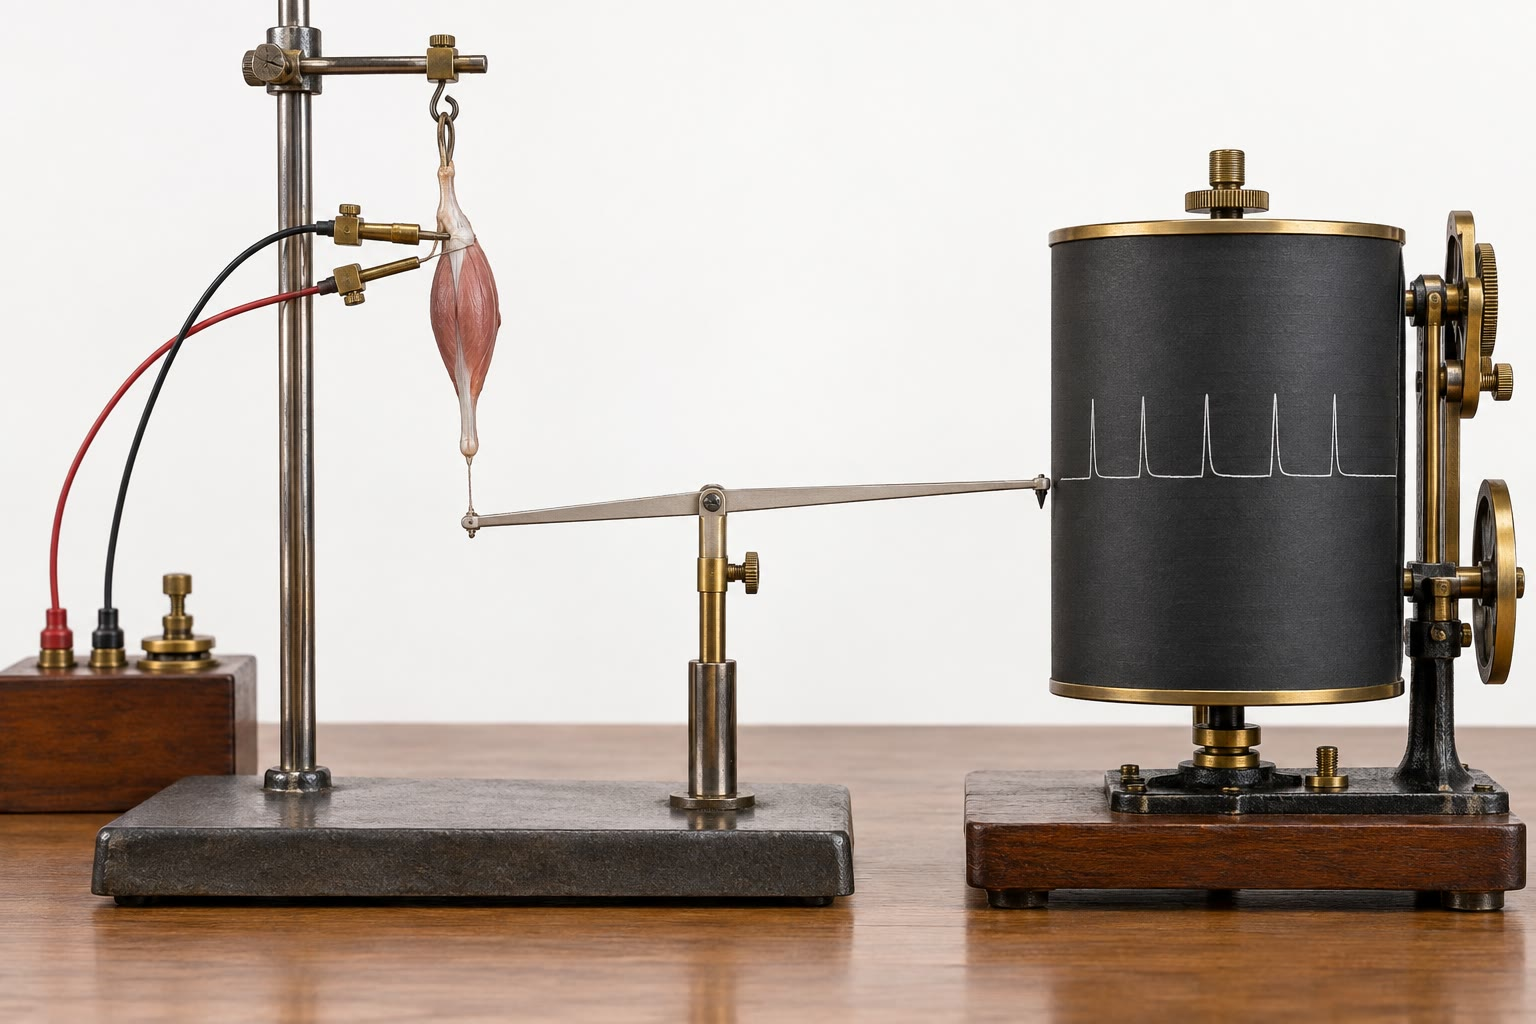
\includegraphics[width=0.44\linewidth]{images/book4/ai/b4-21-frog-muscle-prep.jpg}\hspace{0.04\linewidth}
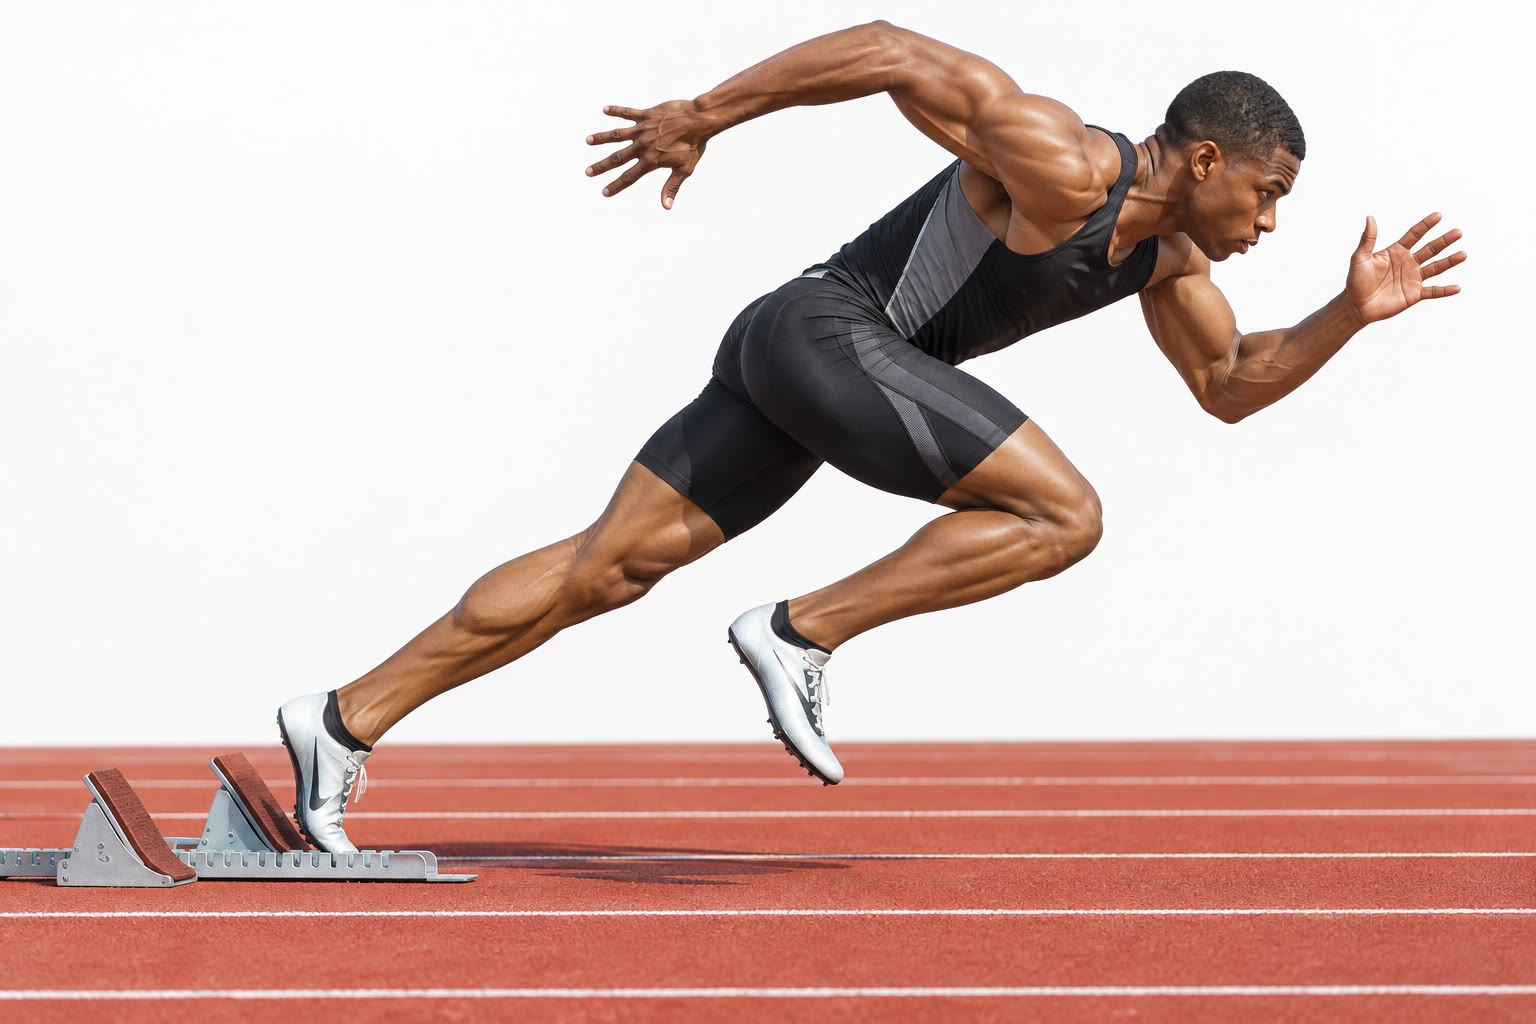
\includegraphics[width=0.44\linewidth]{images/book4/ai/b4-21-sprinter.jpg}

{\small 左：经典标本——蛙的肌肉、其
神经、刺激电极，以及在烟熏鼓上描记的杠杆——
\omterm{def:b2:muscle-movement:motorunit}{单收缩}、叠加与\omterm{def:b2:muscle-movement:motorunit}{强直收缩}正是在此装置上首次记录的。
右：同样的生理现象，肌肉处于充分拉伸状态。}
\end{omfigure}

\section{燃料与疲劳}

\begin{proposition}[做功的供能]\label{prop:b2:muscle-movement:energy}
\index{磷酸肌酸}\index{肌肉疲劳}\index{氧债}
一条\omterm{def:b2:cell-differentiation:myogenesis}{肌纤维}所含的 ATP 只够全力收缩一到两秒。第一种
储备是\emph{\omterm{prop:b2:muscle-movement:energy}{磷酸肌酸}}，它能在毫秒内使 ADP 重新磷酸化，
持续约十秒，是短跑运动员的燃料。
第二种是\omterm{def:b2:cell-differentiation:myogenesis}{肌纤维}糖原的\emph{糖酵解}，
无需氧气，每分子葡萄糖产生两个 ATP 和乳酸：速度快，
可维持一两分钟，并随酸与磷酸基团的
积累而自行受限。第三种是葡萄糖与脂肪酸在线粒体中的\emph{氧化}代谢，
每分子葡萄糖可产生三十个 ATP，其速率受限于
\omterm{def:b2:blood-circulation:blood}{血液}所输送的氧气量，
（见\cref{ch:b2:blood-pressure}）：即马拉松。快速糖酵解型纤维
依赖前两种供能，约一分钟即疲劳；慢速氧化型纤维，
因富含肌红蛋白而呈红色、线粒体丰富，可持续运动数小时。
短时间用力时的\emph{疲劳}并非 ATP 耗尽——
否则肌肉将进入僵直状态——而是
磷酸基团与质子的积累，它们削弱横桥及
钙的释放；长时间用力时则是糖原耗尽，
最终还有意志的耗竭。用力之后，肌肉偿还
其\emph{\omterm{prop:b2:muscle-movement:energy}{氧债}}：恢复\omterm{prop:b2:muscle-movement:energy}{磷酸肌酸}，
将乳酸转回（在肝脏中）并补充其储备，
静止后仍需喘息数分钟。
\end{proposition}

\begin{example}[一百米]\label{ex:b2:muscle-movement:sprint}
以 \qty{20}{kg} 的腿部肌肉、\qty{100}{W/kg} 的功率全力发力十秒，
机械功率为 \qty{2}{kW}；按 \qty{25}{\%} 的效率计算，
ATP 的周转功率为 \qty{8}{kW}——即每秒约 \qty{160}{mmol} 的 ATP，
整场冲刺共消耗 \qty{800}{g} 的 ATP。
肌肉中仅储存约五十克 ATP；\omterm{prop:b2:muscle-movement:energy}{磷酸肌酸}供应最初的
五秒，其余时间由糖酵解承担，这位短跑运动员冲刺结束时
\omterm{def:b2:blood-circulation:blood}{血液}中乳酸浓度达到 \qty{15}{mmol/L}，她需要在随后的
十五分钟内逐步偿还这笔\omterm{prop:b2:muscle-movement:energy}{氧债}。一名马拉松选手以 \qty{300}{W} 的功率跑了两
小时，做功 \qty{2}{MJ}，消耗 \qty{8}{MJ} 的燃料——相当于一千克
糖原与脂肪——氧气以 \qty{4}{L/min} 的速率
全程供给，她在第三十公里处撞上的那堵“墙”，
正是糖原耗尽之处。
\end{example}

\section{练习}

\begin{exercise}[$\star$]\label{exo:b2:muscle-movement:1}
说明肌丝滑行机制，并指出\omterm{def:b2:cell-differentiation:fibre}{肌节}中的哪些带
在收缩时发生变化、哪些不变。
\end{exercise}

\begin{exercise}[$\star$]\label{exo:b2:muscle-movement:2}
写出\omterm{prop:b2:muscle-movement:crossbridge}{横桥循环}的四个步骤，以及 ATP 在每一步中
的作用。为什么没有 ATP 的肌肉会变得僵硬？
\end{exercise}

\begin{exercise}[$\star$]\label{exo:b2:muscle-movement:3}
列出从运动神经冲动到\omterm{prop:b2:muscle-movement:crossbridge}{肌球蛋白}头部附着之间的各个事件，
并给出每一步所需的时间。
\end{exercise}

\begin{exercise}[$\star$]\label{exo:b2:muscle-movement:4}
定义\omterm{def:b2:muscle-movement:motorunit}{运动单位}、\omterm{def:b2:muscle-movement:motorunit}{单收缩}和\omterm{def:b2:muscle-movement:motorunit}{强直收缩}，并给出
神经系统对力量分级的两种方式。
\end{exercise}

\begin{exercise}[$\star\star$]\label{exo:b2:muscle-movement:5}
一个长 \qty{2.4}{\micro m} 的\omterm{def:b2:cell-differentiation:fibre}{肌节}缩短至 \qty{2.0}{\micro m}，
耗时 \qty{50}{ms}。计算细肌丝相对于粗肌丝的
滑动速度；若步长为 \qty{10}{nm}，求
每个附着头部每秒必须完成的循环次数。
\end{exercise}

\begin{exercise}[$\star\star$]\label{exo:b2:muscle-movement:6}
一根长 \qty{10}{cm} 的\omterm{def:b2:cell-differentiation:myogenesis}{肌纤维}含 \num{40000} 个串联的\omterm{def:b2:cell-differentiation:fibre}{肌节}，
在 \qty{0.1}{s} 内缩短 \qty{20}{\%}。计算其缩短速度，
分别以每秒的\omterm{def:b2:cell-differentiation:fibre}{肌节}长度数和米每秒表示，并求
每个\omterm{def:b2:cell-differentiation:fibre}{肌节}的速度。
\end{exercise}

\begin{exercise}[$\star\star$]\label{exo:b2:muscle-movement:7}
利用希尔关系式，取 $a = F_0/4$、$v_{\max} = 10$ 个长度每秒，
计算速度分别为 1、3 和 6 个长度每秒时的力（以 $F_0$ 的比例表示），
以及各速度下的功率，并指出功率在何处最大。
\end{exercise}

\begin{exercise}[$\star\star$]\label{exo:b2:muscle-movement:8}
股四头肌的截面积为 \qty{80}{cm^2}，取 \qty{30}{N/cm^2}，
计算其最大等长收缩力。该肌肉作用于距膝关节 \qty{5}{cm} 处的
一根杠杆，杠杆的脚端距关节 \qty{45}{cm}：
脚端能施加多大的力？
\end{exercise}

\begin{exercise}[$\star\star$]\label{exo:b2:muscle-movement:9}
\omterm{def:b2:muscle-movement:motorunit}{单收缩}的钙脉冲持续 \qty{30}{ms}。解释为什么
\qty{10}{Hz} 的冲动产生波动的力，\qty{50}{Hz} 的冲动产生平滑的\omterm{def:b2:muscle-movement:motorunit}{强直收缩}，
以及为什么\omterm{def:b2:muscle-movement:motorunit}{强直收缩}的力大于\omterm{def:b2:muscle-movement:motorunit}{单收缩}的力。
\end{exercise}

\begin{exercise}[$\star\star\star$]\label{exo:b2:muscle-movement:10}
短跑运动员的 \qty{20}{kg} 腿部肌肉以 \qty{2}{kW} 的功率持续工作，
历时 \qty{10}{s}，效率为 \qty{25}{\%}。计算消耗的 ATP（\qty{50}{kJ/mol}），
覆盖最初 \qty{5}{s} 所需的\omterm{prop:b2:muscle-movement:energy}{磷酸肌酸}量，
以及覆盖其余时间所需\omterm{def:b2:microbial-metabolism:fermentation}{发酵}的葡萄糖量（每个葡萄糖产生 2 个 ATP）。
这些葡萄糖会使 \qty{40}{L} 体液中的乳酸浓度达到多少？
\end{exercise}

\begin{exercise}[$\star\star\star$]\label{exo:b2:muscle-movement:11}
预测以下情况对收缩的影响：一种阻断\omterm{def:b2:cell-differentiation:fibre}{肌质网}
钙释放通道的药物；一种阻断其泵的药物；一个
使\omterm{prop:b2:muscle-movement:coupling}{肌钙蛋白}对钙不敏感的\omterm{def:b2:genome-diversification:mutation}{突变}；以及
从\omterm{def:b2:blood-circulation:blood}{血液}中清除钙，分别针对骨骼肌和心肌。
\end{exercise}

\begin{exercise}[$\star\star\star$]\label{exo:b2:muscle-movement:12}
“肌肉是一台将化学能转化为力的机器，
效率堪比优良的发动机，控制能力堪比计算机。”请讨论其效率（四分之一至二分之一）、
限制效率的因素，
以及神经系统的两种力量分级方式能换来
单一开关无法提供的好处。
\end{exercise}

\section{问题：跳跃的生理学}

\begin{problem}[{周末问题——从肌节到起跳的站立式跳跃分析：
滑动、横桥、钙开关、力–速度极限、
运动单位与燃料，最后求横桥冲程数、
起跳速度时的力，
以及跳跃所耗的 ATP}]
\label{pb:b2:muscle-movement:1}
一人体重 \qty{70}{kg}，竖直向上跳起 \qty{40}{cm}，
使身体质心升高 \qty{0.4}{m}，推动历时 \qty{0.3}{s}。
腿部伸肌（肌肉重 \qty{20}{kg}）的合计
截面积为 \qty{500}{cm^2}，取 \qty{30}{N/cm^2}；其\omterm{def:b2:cell-differentiation:myogenesis}{肌纤维}
长 \qty{12}{cm}（含 \num{48000} 个\omterm{def:b2:cell-differentiation:fibre}{肌节}），推动期间缩短
\qty{4}{cm}；关节将肌肉的缩短量
在脚端放大 \num{10} 倍，力则除以
同一倍数。$v_{\max} = 8$ 个长度每秒，$a = F_0/4$。每根
粗丝携带 \num{300} 个\omterm{prop:b2:muscle-movement:crossbridge}{肌球蛋白}头部；每平方厘米肌肉中有 $6\times
10^{10}$ 根粗丝；每次冲程
长 \qty{10}{nm}，消耗一个 ATP（\qty{8e-20}{J}，\qty{50}{kJ/mol}）；
效率为 \qty{40}{\%}。肌肉中储存 \qty{5}{mmol/kg} 的 ATP 和
\qty{20}{mmol/kg} 的\omterm{prop:b2:muscle-movement:energy}{磷酸肌酸}。\omterm{def:b2:cell-differentiation:myogenesis}{肌纤维}直径为 \qty{60}{\micro
m}。\omterm{def:b2:muscle-movement:motorunit}{运动单位}：每个肌群含 \num{800} 个，每个含 \num{50} 至
\num{2000} 根\omterm{def:b2:cell-differentiation:myogenesis}{肌纤维}。

\medskip
\noindent\textbf{第一部分——力学。}
\begin{enumerate}
  \item 计算升高 \qty{40}{cm} 所需的起跳速度，
        （$v^{2} = 2gh$），并求起跳时的动能。
  \item 计算双腿在蹬地过程中对地面施加的平均力（
        蹬地距离为 \qty{0.4}{m}，所做的功等于动能加上克服重力所做的功），
        并与体重相比较。
  \item 计算伸肌的最大等长收缩力，并
        以杠杆比 10 计算其能给出的
        最大足部作用力。
  \item 计算纤维的缩短速度，以每秒的长度数表示，
        并求其占 $v_{\max}$ 的比例。
  \item 利用 Hill 关系式，计算该速度下可用的力，
        占 $F_0$ 的比例，以及由此得到的足部作用力。
        能否仅靠肌肉完成起跳？其余的
        力从何而来？
  \item 计算蹬地过程中的平均机械功率，
        以及每千克伸肌的功率。
\end{enumerate}

\medskip
\noindent\textbf{第二部分——横桥。}
\begin{enumerate}[resume]
  \item 每个\omterm{def:b2:cell-differentiation:fibre}{肌节}缩短多少，沿每根半\omterm{def:b2:cell-differentiation:fibre}{肌节}需要完成多少次
        \qty{10}{nm} 的摆动，
        才能使其细丝滑动这一距离？
  \item 计算每根半\omterm{def:b2:cell-differentiation:fibre}{肌节}中的滑动速度，以及
        若某一头部持续附着，它每秒将完成的
        摆动次数。
  \item 计算伸肌中\omterm{prop:b2:muscle-movement:crossbridge}{肌球蛋白}头部的数目。
  \item 计算肌肉本身所做的功（即其在起跳速度下的力
        乘以其缩短量），每次摆动在
        \qty{40}{\%} 效率下所做的功，以及所需的摆动次数。
  \item 这相当于每个头部需要多少次摆动，
        与第 7 题中可用的次数相比如何？请对此储备加以评述。
  \item 计算起跳所消耗的 ATP，分别以摩尔和克
        （\qty{507}{g/mol}）表示，并由该 ATP 所含能量
        校核效率。
\end{enumerate}

\medskip
\noindent\textbf{第三部分——开关与指令。}
\begin{enumerate}[resume]
  \item 蹬地历时 \qty{0.3}{s}，单次冲动的钙脉冲历时
        \qty{30}{ms}。何种放电频率能使纤维保持
        \omterm{def:b2:muscle-movement:motorunit}{强直收缩}？每个运动\omterm{def:b2:neurons-synapses:neuron}{神经元}发出多少个冲动？
  \item 游离钙浓度从 \qty{0.1}{} 升至 \qty{10}{\micro
        mol/L}，纤维体积为 \qty{5e-10}{L}。这涉及多少个游离钙离子？
        将其泵回所需的泵循环数
        是多少（每个 ATP 转运两个离子）？
  \item 计算伸肌中的纤维数，以及每个纤维每次冲动所耗的
        横桥 ATP，并与第 14 题中的泵耗能相比较。
        真实的泵运耗能约占肌肉 ATP 的四分之一：
        游离钙的测定
        低估了什么？
  \item 神经系统按大小\omterm{def:b2:muscle-movement:motorunit}{募集}\omterm{def:b2:muscle-movement:motorunit}{运动单位}。起跳时，
        哪些\omterm{def:b2:muscle-movement:motorunit}{运动单位}被\omterm{def:b2:muscle-movement:motorunit}{募集}，以何种顺序进行？
        轻柔的一步会用到 \num{800} 个中的多大比例？
  \item 解释为何在用力较小时力可以精细分级，
        而接近最大值时只能粗略分级。
  \item 某人服用一种能将\omterm{prop:b2:neurons-synapses:integration}{神经肌肉接头}的传递阻断一半的药物，
        预测其\omterm{def:b2:muscle-movement:motorunit}{单收缩}、\omterm{def:b2:muscle-movement:motorunit}{强直收缩}和起跳的情况。
\end{enumerate}

\medskip
\noindent\textbf{第四部分——燃料。}
\begin{enumerate}[resume]
  \item 计算伸肌中储存的 ATP，并与
        起跳的消耗量相比较。
  \item 计算\omterm{prop:b2:muscle-movement:energy}{磷酸肌酸}储备，以及它能支付的
        起跳次数。
  \item 连续起跳十次：哪种燃料接替供能，以及
        何种物质会累积？
  \item \omterm{def:b2:blood-circulation:blood}{血液}每分钟可向伸肌输送 \qty{2}{L} 氧气，
        （每个 $\mathrm{O_2}$ 对应 6 个 ATP）。起跳功率需要多大的 ATP 周转速率，
        以及这需要多少氧气供应？
        得出结论。
  \item 起跳之后，此人剧烈呼吸一分钟。
        计算再合成所用\omterm{prop:b2:muscle-movement:energy}{磷酸肌酸}和 ATP 所需的氧气量
        （每个 $\mathrm{O_2}$ 分子对应 \qty{6}{ATP}），
        并与静息时的耗氧量
        （\qty{250}{mL/min}）相比较。
  \item 为何跳跃者的肌肉在 ATP 如此快速周转的情况下，
        仍不会进入僵直状态？
  \item 陈述结论：每根半\omterm{def:b2:cell-differentiation:fibre}{肌节}的摆动次数，起跳速度下的力
        所占的比例，以及起跳所消耗的 ATP。
\end{enumerate}
\end{problem}
